\newgeometry{hmargin = 4mm, vmargin = 2cm}
\thispagestyle{empty}
\begin{landscape}
	\section{LTI-Grundglieder \formelbuch{115 \& 201}}
	\begin{table}[h!]
		\usetikzlibrary{arrows}
		\usetikzlibrary{positioning}
		\usetikzlibrary{decorations.markings}
		\usetikzlibrary{decorations.pathreplacing}
		\tikzset{
			font = \small,
			axis/.style = {
				thick, ->
			},
			locus/.style = {
				ultra thick, hsr-blue,
				postaction = {
					decorate, decoration = {
						markings,
						mark = between positions .2 and .92 step 6mm  with {%
							\draw[ultra thick, ->] (0,0) -- ++(1pt,0);
						},
					},
				},
			},
			dot/.style = {
				circle, draw = hsr-blue, thick,
				fill = white,
				inner sep = 0pt,
				minimum size = 1mm,
			},
			indbrace/.style = {
				gray,
				thick,
				decorate,
				decoration = {
					brace,
					raise = 5pt,
				},
			},
		}
		\centering
		\begin{tabularx}{\linewidth}{%
				c >{\centering}m{4cm}%
				*{2}{ >{\(\displaystyle}c<{\)} }%
				m{3.5cm} m{4cm} X%
		}
			\toprule[2pt]

			\bfseries Typ &
			\bfseries Symbol &
			\textbf{Differentialgleichung} &
			\textbf{Frequenzgang } G &
			\bfseries Nyquistdiagramm &
			\bfseries Bodediagramm &
			\bfseries Anmerkungen \\

			\midrule[1pt]

			%
			% Proportional
			%
			P &
			\begin{tikzpicture}
				\node[rtprop] (G) {};
				\node[anchor = south west] at (G.north west) {\(K\)};
				\draw[ultra thick, ->] (G.west) ++(-.5,0) node[left] {\(u\)} -- (G.west);
				\draw[ultra thick, ->] (G.east) -- ++(.5,0) node[right] {\(y\)};
			\end{tikzpicture}
			&
			y = Ku & K
			&
			\begin{tikzpicture}
				\draw[axis] (-.2,0) -- (1.8,0) node[right] {Re};
				\draw[axis] (0,-.5) -- (0,.3) node[above] {Im};
				\coordinate (P) at (1.5,0);
				\draw[indbrace] (P) -- node[midway, below = 7pt] {\(K\)} (0,0);
				\node[dot] at (P) {};
			\end{tikzpicture}
			\\

			\midrule[1pt]

			%
			% Delay
			%
			T &
			\begin{tikzpicture}
				\node[rtdelay] (G) {};
				\node[anchor = south east] at (G.north east) {\(T_t\)};
				\draw[ultra thick, ->] (G.west) ++(-.5,0) node[left] {\(u\)} -- (G.west);
				\draw[ultra thick, ->] (G.east) -- ++(.5,0) node[right] {\(y\)};
			\end{tikzpicture}
			&
			y(t) = \varepsilon(t) u(t - T_t) & e^{-j\omega T_t}
			&
			\begin{tikzpicture}
				\draw[axis] (-1,0) -- (1,0) node[right] {Re};
				\draw[axis] (0,-1) -- (0,1) node[above] {Im};
				\draw[locus] (.75,0) arc (360:0:.75);
				\node[dot] at (.75,0) {};
				\node[below right = .5mm] at (.75,0) {\(\omega = 2\pi n\)};
			\end{tikzpicture}
			\\

			\midrule[1pt]

			%
			% PT1
			%
			PT\(_1\) &
			\begin{tikzpicture}
				\node[rtpt1] (G) {};
				\node[anchor = south west] at (G.north west) {\(K\)};
				\node[anchor = south east] at (G.north east) {\(T\)};
				\draw[ultra thick, ->] (G.west) ++(-.5,0) node[left] {\(u\)} -- (G.west);
				\draw[ultra thick, ->] (G.east) -- ++(.5,0) node[right] {\(y\)};
			\end{tikzpicture}
			&
			T\dot{y} + y = Ku & \frac{K}{j\omega T + 1}
			&
			\begin{tikzpicture}
				\draw[axis] (-.2,0) -- (1.8,0) node[right] {Re};
				\draw[axis] (0,-1) -- (0,.6) node[above] {Im};
				\draw[locus] (1.5,0) arc (360:180:.75);
				\draw[indbrace] (0,0) -- node[midway, above = 7pt] {\(K\)} (1.5,0);
				\draw
					(0,0) node[dot] {} % node[above left, anchor = south east] {\(\omega\to\infty\)}
					(1.5,0) node[dot] {} node[above right = 2pt, anchor = south west] {\(\omega = 0\)} 
					(.75,-.75) node[dot] {} node[below] {\(\omega = 1/T\)}
				;
			\end{tikzpicture}
			\\

			\midrule[1pt]

			%
			% PT2
			%
			PT\(_2\) &
			\begin{tikzpicture}
				\node[rtpt2] (G) {};
				\node[anchor = south west] at (G.north west) {\(K\)};
				\node[anchor = south] at (G.north) {\(\zeta\)};
				\node[anchor = south east] at (G.north east) {\(T\)};
				\draw[ultra thick, ->] (G.west) ++(-.5,0) node[left] {\(u\)} -- (G.west);
				\draw[ultra thick, ->] (G.east) -- ++(.5,0) node[right] {\(y\)};
			\end{tikzpicture}
			&
			T^2 \ddot{y} + 2\zeta T \dot{y} + y = Ku &
			\frac{K}{T^2 (j\omega)^2 + 2\zeta T (j\omega) + 1} 
			&
			\begin{tikzpicture}
				\draw[axis] (-.2,0) -- (1.8,0) node[right] {Re};
				\draw[axis] (0,-1) -- (0,.6) node[above] {Im};

				\draw[locus] (1.5,0) 
					to[out = -90, in = 0] (.75,-.8)
					to[out = 180, in = -30] (0, -.7)
					to[out = 160, in = 190] (0,0)
				;

				\draw[indbrace] (0,0) -- node[midway, above = 7pt] {\(K\)} (1.5,0);
				\draw
					(0,0) node[dot] {} % node[above left, anchor = south east] {\(\omega\to\infty\)}
					(1.5,0) node[dot] {} node[above right = 2pt, anchor = south west] {\(\omega = 0\)} 
					(0,-.7) node[dot] {} node[below left = 4pt, anchor = north west] {\(\omega = 1/T\)}
				;
			\end{tikzpicture}
			\\

			\midrule[1pt]

			%
			% Integrator
			%
			I &
			\begin{tikzpicture}
				\node[rtint] (G) {};
				\node[anchor = south west] at (G.north west) {\(K\)};
				\draw[ultra thick, ->] (G.west) ++(-.5,0) node[left] {\(u\)} -- (G.west);
				\draw[ultra thick, ->] (G.east) -- ++(.5,0) node[right] {\(y\)};
			\end{tikzpicture}
			&
			\dot{y} = K u & \frac{K}{j\omega}
			&
			\begin{tikzpicture}
				\draw[axis] (-.2,0) -- (1.8,0) node[right] {Re};
				\draw[axis] (0,-1) -- (0,.3) node[above] {Im};

				\draw[locus] (0,-1) -- (0,0);
				\draw
					(0,0) node[dot] {} node[above right = 2pt] {\(\omega\to\infty\)}
					(0,-.5) node[dot] {} node[left] {\(j\)}
				;
			\end{tikzpicture}
			\\

			\midrule[1pt]

			%
			% Proportional with Integrator
			%
			PI &
			\begin{tikzpicture}
				\node[rtpi] (G) {};
				\node[anchor = south west] at (G.north west) {\(K\)};
				\node[anchor = south east] at (G.north east) {\(T\)};
				\draw[ultra thick, ->] (G.west) ++(-.5,0) node[left] {\(u\)} -- (G.west);
				\draw[ultra thick, ->] (G.east) -- ++(.5,0) node[right] {\(y\)};
			\end{tikzpicture}
			&
			y = K_R \left( u + \int_0^t \frac{u ~d\tau}{T} \right) &
			K \left( 1 + \frac{1}{j\omega T} \right)
			&
			\begin{tikzpicture}
				\draw[axis] (-.2,0) -- (1.8,0) node[right] {Re};
				\draw[axis] (0,-1) -- (0,.4) node[above] {Im};

				\draw[locus] (.7,-1) -- (.7,0);
				\draw[indbrace] (0,0) -- node[midway, above = 7pt] {\(K\)} (.7,0);
				\draw
					(.7,0) node[dot] {} node[above right = 2pt] {\(\omega\to\infty\)}
				;
			\end{tikzpicture}
			\\

			\midrule[1pt]

			%
			% Differentiator
			%
			D &
			\begin{tikzpicture}
				\node[rtdiff] (G) {};
				\node[anchor = south west] at (G.north west) {\(K\)};
				\draw[ultra thick, ->] (G.west) ++(-.5,0) node[left] {\(u\)} -- (G.west);
				\draw[ultra thick, ->] (G.east) -- ++(.5,0) node[right] {\(y\)};
			\end{tikzpicture}
			&
			y = K\dot{u} & j\omega K
			&
			\begin{tikzpicture}
				\draw[axis] (-.2,0) -- (1.8,0) node[right] {Re};
				\draw[axis] (0,-.3) -- (0,1) node[above] {Im};

				\draw[locus] (0,0) -- (0,1);
				\draw
					(0,0) node[dot] {} node[below right = 2pt] {\(\omega = 0\)}
				;
			\end{tikzpicture}
			&
			&
			Nicht realisierbar.
			\\

			\midrule[1pt]

			%
			% Real differentiator
			%
			DT\(_1\) &
			\begin{tikzpicture}
				\node[rtdt1] (G) {};
				\node[anchor = south west] at (G.north west) {\(K\)};
				\node[anchor = south east] at (G.north east) {\(T\)};
				\draw[ultra thick, ->] (G.west) ++(-.5,0) node[left] {\(u\)} -- (G.west);
				\draw[ultra thick, ->] (G.east) -- ++(.5,0) node[right] {\(y\)};
			\end{tikzpicture}
			&
			T\dot{y} + y = K\dot{u} & \frac{j\omega K}{1 + j\omega T}
			&
			\begin{tikzpicture}
				\draw[axis] (-.2,0) -- (1.8,0) node[right] {Re};
				\draw[axis] (0,-.5) -- (0,1.1) node[above] {Im};
				\draw[locus] (0,0) arc (180:0:.75);
				\draw[indbrace] (1.5,0) -- node[midway, below = 7pt] {\(K\)} (0,0);
				\draw
					(0,0) node[dot] {}
					(1.5,0) node[dot] {} node[below right = 2pt, anchor = north west] {\(\omega = 0\)} 
					(.75,.75) node[dot] {} node[above] {\(\omega = 1/T\)}
				;
			\end{tikzpicture}
			\\

			\bottomrule[2pt]
		\end{tabularx}
	\end{table}
\end{landscape}
\restoregeometry

\subsection{\"Aquivalente Glieder}

\subsection{PT\(_2\)--Glied}
\subsubsection{D\"ampfung}
\subsubsection{Ersatzmodell}

\subsubsection{Parameter der Sprungantwort}
\renewcommand{\arraystretch}{1.8}
\begin{tabular}{|m{7cm}|m{1cm}m{0.5cm}m{8cm}}
  \cline{1-1}
  $y_{\infty} =A \cdot K$ & &
  $y_{\infty}$: & Endwert\\
  \cline{1-1}  
	$T_\omega = 2T_m=\dfrac{2\pi}{\omega_n \sqrt{1-\zeta^2}}=\dfrac{2\pi}{\omega}$ & &
	$T_{\omega}$: & Schwingungsdauer \\
  \cline{1-1}
	$\varepsilon = \dfrac{\Delta y}{y_{\infty}}$ & &
	\parbox{0.5cm}{
		$\varepsilon$:\\
		$\Delta y$:
	} & 
	\parbox{8cm}{
		Verhältnis von Überschwinger nach $T_e$ zum Endwert\\
		Toleranzbereich der Amplitude nach $T_e$
	}\\
  \cline{1-1}  
	$T_e = \dfrac{\ln\left(\varepsilon\sqrt{1-\zeta^2}\right)}{-\omega_n\cdot\zeta} = 
	\dfrac{1}{\sigma}\ln\left(\dfrac{\varepsilon\omega}{\omega_n}\right)$ & &
	$T_e$: & Einschwingzeit \\
  \cline{1-1}  
	$T_m = \dfrac{\pi}{\omega_n\sqrt{1-\zeta^2}}=\dfrac{\pi}{\omega}$ & &
	$T_m$: & Überschwingungsdauer\\
  \cline{1-1}  
	$y_m = y_{\infty} \cdot e^{\frac{-\pi\cdot\zeta}{\sqrt{1-\zeta^2}}}$ & &
	$y_m$: & Überschwingweite\\
   \cline{1-1}  
	$\omega = \dfrac{1}{T}\sqrt{1-\zeta^2}= \omega_n\sqrt{1-\zeta^2}=\dfrac{2\pi}{T_\omega}=2\pi f$ & &
	$\omega$: & Kreisfrequenz \\
  \cline{1-1}  
	$\omega_n = \dfrac{1}{T}$ & &
	$\omega_n$: & Kennkreisfrequenz \\
  \cline{1-1}  
	$T_a = \frac{\pi - \arccos{(\zeta)}}{\omega_n\cdot\sqrt{1-\zeta^2}}$ & &
	$T_a$: & Anschwingzeit/Anregelzeit \\
  \cline{1-1}  
	$\sigma = -\dfrac{\zeta}{T} = -\zeta\omega_n$ & &
	$\zeta$: & Dämpfungskonstante \\
  \cline{1-1}
	$\delta = \ln{\Big(\frac{y_i}{y_{i+1}}\Big)} = \frac{2\pi \zeta}{\sqrt{1-\zeta^2}}$ & &
	$\delta$: & Logarithmisches Dekrement\\
  \cline{1-1}  
\end{tabular}
\renewcommand{\arraystretch}{1}
	
\subsubsection{Sprungantwort}
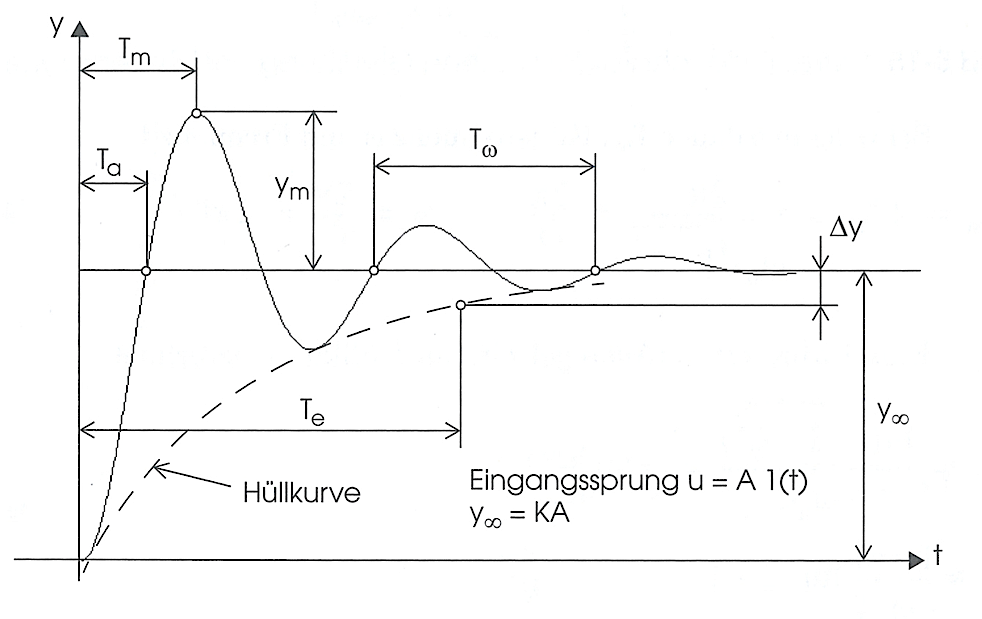
\includegraphics[width = 9cm]{./images/pt2StepResp}

\subsubsection{Dämpfung}
Optimal bei $\zeta=\frac{1}{\sqrt{2}}$ ($\Psi=45$).
Dabei erreicht die Regelgrösse $y$ nach $4.3\%$ Überschwingen rasch den	Endwert.

\subsubsection{Berechnung $\zeta$}
\textbf{Aus DGL} $\ddot{y}+a_1\dot{y}+a_0 y=\ldots$ folgt $a_1=2\zeta\omega_n$, 
$a_0=\omega_n^2$
$\Rightarrow \zeta=\frac{a_1}{2\sqrt{a_0}}$ \\
\textbf{Mittels Überschwingweite} kann $\zeta$ ebenfalls berechnet werden\\
\begin{tabular}{p{2.5cm}p{2.5cm}p{4cm}}
$\zeta = \frac{1}{\sqrt{1+(\frac{\pi}{c})^2}}$ & $c =ln(\frac{y_m}{y_{\infty}})$ & $y_m$: Überschwingweite
\end{tabular}

Weitere Formeln in der LTI-Grundglieder Tabelle
